\section{Stockholm Congestion Tax}\label{sec:stockholm}

\subsection{Implementation\protect\footnote{This history is based on \citet{Eliasson2009b} and \citet{GullbergIsaksson2009}.}}

In 2000, the Swedish parliament set up a ``Stockholm Commission'' to  prioritize infrastructure projects for Stockholm, and directed it to reconsider road pricing as source of funds. As it happened, 2002 was also an election year, and the Moderate Party (Sweden's mainstream conservative party) pounced on the renewed discussion of pricing to win some voters from their rivals, the Social Democrats. In response, a Social Democrat leader, Annika Billstr\"om, announced on television, ``My message to the voters of Stockholm is that there will be no road charging during our next term of office.'' 

The September 2002 election wound up with the Social Democrats and their allies, the Left Party, just short of a majority both nationally and in Stockholm. Seizing the opportunity, the small Green Party made a pact to join the Social Democrat/Left coalition in exchange for a trial of pricing in Stockholm. The deal sparked a public outcry over Annika Billstr\"om's (by then Mayor of Stockholm) broken pledge, and opponents demanded a popular referendum on pricing. The Social Democrats agreed the September 2006 election ballot in Stockholm would include a referendum on whether to make pricing permanent. Originally, the trial was meant to last several years, but political and legal complications delayed the start until January 3, 2006. The trial lasted until July 31, 2006 and was accompanied by a mild transit expansion---mainly bus services--lasting from September 2005 to December 2007 (see \citet{Kottenhoff2009} for analysis).

Prior to the trial, media coverage of the trial was very negative, and polls showed strong opposition. But once the trial began, public opinion shifted quickly in favor due to very visible congestion reductions.\footnote{A small literature now exists on the question of why public opinion shifted---e.g., XXX LIST SOURCES} At the September 2006 elections, 53\% of Stockholm residents voted to make the scheme permanent. However, at the same election, the leftist coalition lost control of the government at all levels to a center-right alliance of parties who opposed pricing---thus throwing the SCT's future into doubt.  But in the end the new government agreed to respect the referendum results after negotiating a \euro 10 billion infrastructure package, whereby toll revenues were matched by national funds to build new roads---as in the Dennis Package. The SCT returned on a permanent basis on August 1, 2007. In January 2016, tolls were increased and geographically extended.

\subsection{Design}

The Stockholm Congestion Tax (SCT) is a time-variable toll on weekday trips in both directions across a cordon around central Stockholm. See Fig. \ref{fig:stockholm-map} for a map of the tolling sites, which are mostly unchanged. The map has labeled a highway called the Essingeleden; this was originally toll-free for political reasons---being the only north-south route around the city---but in January 2016 it became tolled, although at slightly different rates than in the cordon. The SCT is turned off in July, as Swedes have July off work and traffic is light.

During the trial, the SCT used a radio-frequency tag-and-beacon system backed up by ANPR cameras, but with time the error rate for ANPR became low enough that transponder enforcement was ended in late 2008 \citep[p. 841]{Hamilton2011}. Vehicles are charged when they cross under metal gantries, which work as a trio: when a laser on the middle gantry detects a vehicle, cameras mounted on the first and third photograph the front and rear plates.

Figure \ref{fig:stockholm-prices} displays the current charging schedule, alongside that of Gothenburg's. Originally, tolls during the peaks were about 2/3 of their current values, but in 2016 the charge was increased to fund an infrastructure package \citep{Borjesson2018}. Although vehicles are ostensibly charged for each cordon passage, there is a maximum daily charge, beyond which traversals are free; the maximum was 60 SEK until the 2016 toll increase but is now 100 SEK. 

Today, emergency vehicles, diplomatic vehicles, vehicles for disabled person and and buses weighing at least 14 metric tonnes are exempt. Vehicles registered abroad were exempt until 2015. Alternative-fuel vehicles were exempt until 2012. Taxis were exempt only during the trial. Trips going directly between the island of Liding\"o (the starred island in Fig. \ref{fig:stockholm-map}) are exempt, since Liding\"o can only be accessed via the SCT zone. Such direct trips are identified as trips that cross two tolling sites within thirty minutes, with one of the two being among the tolling sites at the Liding\"o. Until recently, companies were allowed to pay the toll for employees driving company cars (about one quarter of cordon crossings) as an untaxed fringe benefit, which, given Sweden's high taxes, significantly diminished the toll; but as of 2018 new legislation has ended this practice \citep[Sec. 2.2]{Borjesson2018}.

\begin{figure}
    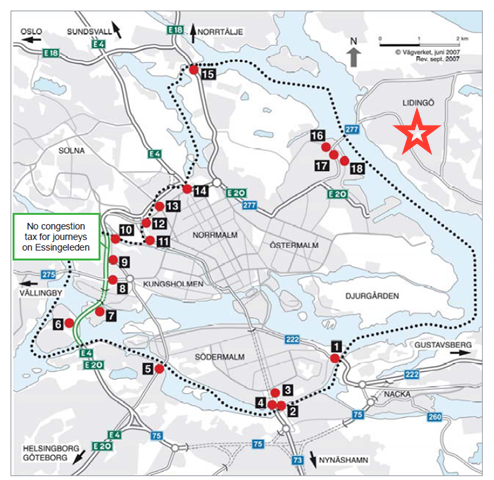
\includegraphics[width=5in]{../img/stockholm-map.png}
    \caption{Stockholm Congestion Tax, access points in red. \citep{transportstyrelsen2015}}
    \label{fig:stockholm-map}
\end{figure}

\begin{figure}
    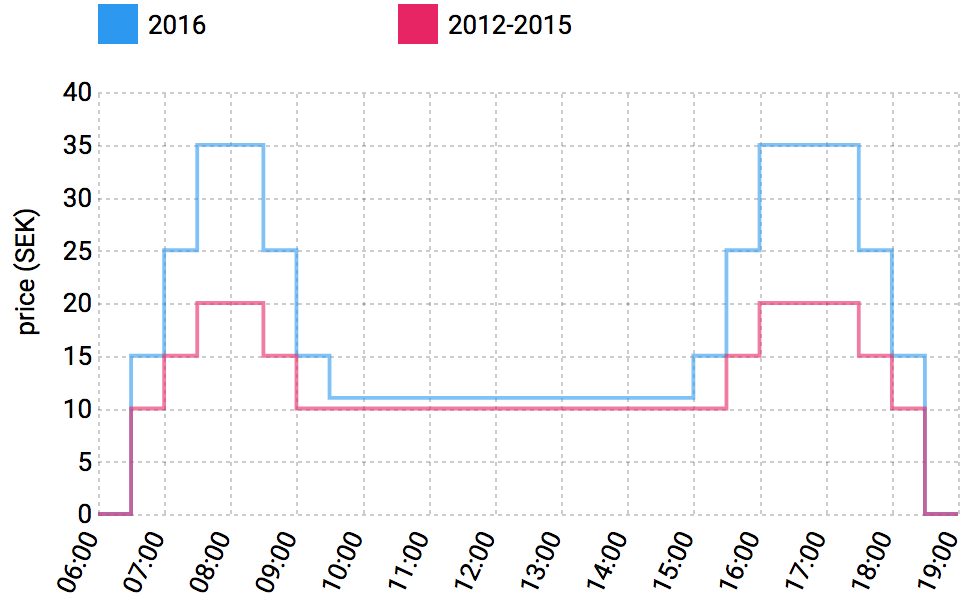
\includegraphics[width=4.5in]{../img/stockholm-prices.png}
    \caption{Stockholm toll schedule }
    \label{fig:stockholm-prices}
\end{figure}

\subsection{Transportation impacts}

During the trial, flows across the cordon during charging hours fell by about 20\% in both the peaks and the mid-day off-peak, exceeding the 16\% drop that had been forecast \citep{Eliasson2013}. After the reintroduction of the charge, and despite growth in Stockholm, cordon flows remained almost constant \citep[Tab. 4]{Borjesson2018}. The share of exempt traffic hovered between 25\% and 28\% from 2008 to 2011, but thereafter declined to about 15\% due to the removal of the exemption for electric vehicles. 

Theme II appears again in that, after the 2016 price increase, cordon traversal  during the peaks fell only 5\%, despite charges almost doubling \citep[p. 43, Tab. 6]{Borjesson2018}. The authors calculate the price elasticity of demand from the charge increase to be only 30\% of the elasticity implied by the introduction of charging.

During the trial, taxis---which were exempt---were expected to account for 4\% of traffic, but actually acounted for 8\% \citep{Eliasson2013}. This result accords with the early experience in Singapore and London, where taxi entries surged.

Using survey data for the trial, \citet{Franklin2008} find the fall in person-trips was similar for commuters (24\%) and discretionary travelers (22\%), but the two groups adapted differently: commuters who stopped driving switched to public transit, while discretionary travelers cancelled or rerouted their trips. 

Travel time savings exceeded forecasts substantially, mainly due to reductions in queues which traffic forecasters had trouble modelling \citep{Eliasson2013}. Figure \ref{fig:stockholm-travel-time} shows delays recorded on different roads; as the figure shows these gains gains persisted over the years they were measured.

\begin{figure}
    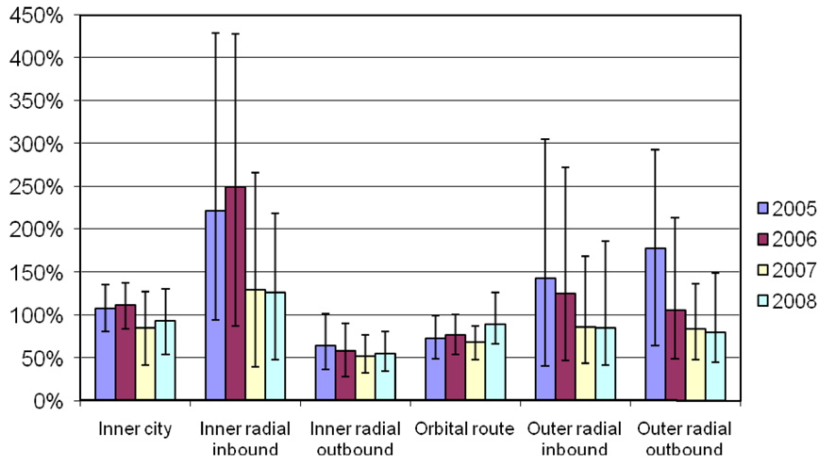
\includegraphics[width=\textwidth]{../img/stockholm-travel-times.png}
    \caption{Sweden price structure \citep{Borjesson2012} XXX INCLUDE NOTE LATER EXPLAINING THE METRIC. Note that the orbital route lies outside the cordon.}
    \label{fig:stockholm-travel-time}
\end{figure}

\citet{Simeonova2017} finds robust evidence that the Congestion Tax caused a 5-10 percent decline in air pollution, which led to a 47\% fall in the rate of urgent care visits for children with asthma.

\subsection{Finances}

The cost of the charging system trial was 1900 MSEK, of which 1050 MSEK was spent prior to the start of charging \citep{Eliasson2009}. Another 1400 MSEK paid for the public transit expansion---mostly to buy 200 buses and run extra bus lines until December 2007 \citep[p. 398]{Eliasson2008}.

\citet{Hamilton2011} describes several factors that explains the high cost of implementation. First, transaction costs were originally high because every charge was processed separately. Second, the Liding\"o exemption required an expensively low false negative rate (achieved by manually double-checking video), because if the system identifies a Liding\"o trip when it enters the cordon but misses it leaving (or vice versa), then it charges the exempt trip.\footnote{Jones Eliason, a researcher involved in the implementation, has remarked, ``Had we realized just how expensive the Liding\"o exception would be, it is unlikely that it would have been adopted'' \citep[p. 217]{Eliasson2009b}.} Third, delay caused by legal and political complications wasetd contractors' time. Finally, having such a short trial required expensive redundancy and overdesign, because the system had to work perfectly and immediately with little testing.


 SCT has since become very profitable. In 2008, operating costs were 220 MSEK and revenues 710 MSEK, but by 2016 operating costs were down to 103 MSEK and revenues up to 1400 MSEK \citep[p. 40]{Borjesson2018}. Revenues during the trial were 14\% less than expected, which \citet{Eliasson2013} explain is partly due to underestimating the fall in demand but mainly due to a higher-than-expected share of exempt traffic.
